\documentclass[12pt, a4paper]{article}
\title{Industrial Training Report}
\usepackage{hyperref}
\usepackage{tabularx}
\usepackage{graphicx}
\usepackage{multirow}
\usepackage{longtable}
\usepackage{amsmath}
\usepackage{amsfonts}
\usepackage{amssymb}
\usepackage{amsthm}
\usepackage{eucal}
\usepackage{ragged2e}
\usepackage{upgreek}
\usepackage[margin=1in]{geometry}

\tolerance=1
\emergencystretch=\maxdimen
\hyphenpenalty=10000
\hbadness=10000

\graphicspath{{./images/}}
\author{Manas Khanna}
\date{}

\begin{document}
\thispagestyle{empty}
{\large \begin{center}
  
\includegraphics[width=0.6\textwidth]{logo}\\ \vspace{20px}
  \textbf{Industrial Traning Report}\\ \medskip 
  \small on\\ \medskip
  \normalsize ``\textbf{SUMMARIZATION \& DECISION TRACIBILITY SYSTEM FOR SEMICONDUCTOR PRODUCT DEVELOPMENT LIFECYCLE}'' \\ \medskip
  \small Submitted in partial fulfillment of the requirements for the award of the degree of \\ \medskip
  \normalsize \textbf{BACHELOR OF TECHNOLOGY}\\
in\\
\textbf{COMPUTER SCIENCE AND ENGINEERING}\\
by\\
\begin{tabular}{l c c c r}
\textbf{MANAS KHANNA} & & & & \textbf{A25305223002}
\end{tabular}\\ \bigskip
\textbf{Under the Guidance of\\ \medskip
Ms. Anjali Negi\\ \medskip
(POST)} \\ \begin{center} \end{center}
  {\large AMITY SCHOOL OF ENGINEERING AND TECHNOLOGY}\\
Amity University Punjab\\
Mohali – 140306\\
2026-27\\\end{center}
\newpage
\normalsize
\pagenumbering{roman}
\addcontentsline{toc}{section}{Certificate}
\begin{center}
  \textbf{Certificate}\\
\vspace{10px}
% \fbox{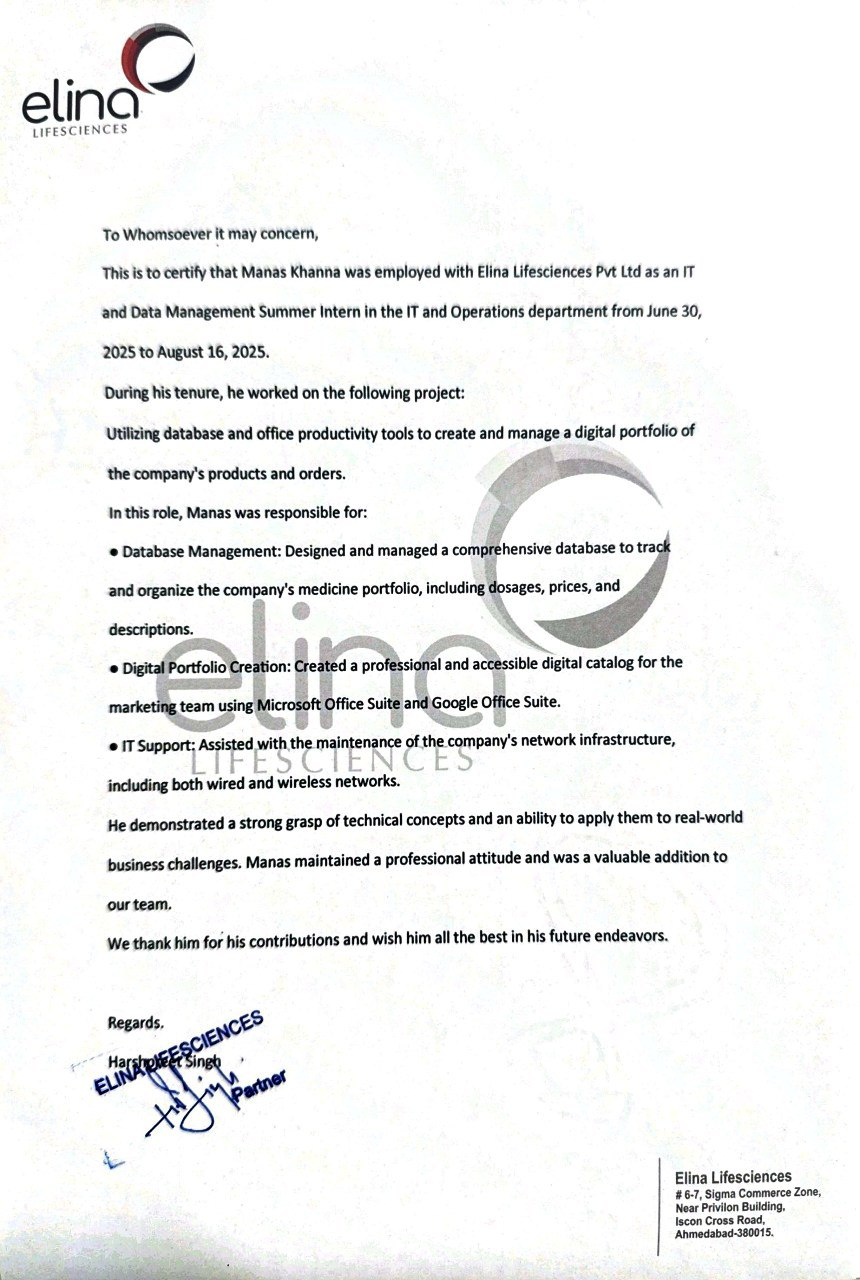
\includegraphics[width=0.7\textwidth]{internship.png}}
\end{center}
\newpage
}

\section*{DECLARATION}
\addcontentsline{toc}{section}{Declaration}
I, \textbf{Manas Khanna}, student of B.Tech in Computer Science and Engineering at Amity University Punjab, hereby declare that the internship work entitled \textbf{``Summarization and Decision Traceability System for Semiconductor Product Development Lifecycle''} has been carried out by me during my industrial training at \textbf{SCL Mohali} under the guidance of \textbf{Mr. Harhspreet Singh}.

This report is submitted in partial fulfillment of the requirements for the award of the degree of Bachelor of Technology in Computer Science and Engineering for the academic session 2026--27.

I further declare that this report is based on the software system, documentation corpus, and implementation work present in the project repository studied during the internship period, and that it has not been submitted elsewhere for the award of any other degree or diploma.

\vspace{2cm}
\noindent Date: \\
\vspace{1cm}
\noindent Place: \\
\vspace{2cm}

\hfill \textbf{Manas Khanna}
\newpage

\section*{ACKNOWLEDGEMENT}
\addcontentsline{toc}{section}{Acknowledgement}
I express my sincere gratitude to my parents for their constant encouragement and support.

I am thankful to \textbf{SCL Mohali} for providing me with an opportunity to work in a disciplined technical environment and for allowing me to study a problem at the intersection of semiconductor program management, document processing, and applied Artificial Intelligence.

I am especially grateful to \textbf{Mr. Harhspreet Singh} for his guidance, feedback, and support throughout the internship. I also thank the technical teams whose workflows, documentation styles, and traceability needs shaped the direction of the work.

I would also like to thank the faculty of Amity School of Engineering and Technology for their encouragement and academic support during the preparation of this report.

\vspace{1cm}
\hfill \textbf{Manas Khanna}
\newpage

\section*{ABSTRACT}
\addcontentsline{toc}{section}{Abstract}
This internship focused on building a local-first web application for organizing engineering documents produced during a semiconductor product development program and converting those documents into structured, searchable knowledge. The implemented system is titled \textbf{Summarization and Decision Traceability System for Semiconductor Product Development Lifecycle}.

The application is built using \textbf{FastAPI}, \textbf{SQLite}, \textbf{SQLAlchemy}, \textbf{Jinja templates}, \textbf{vanilla JavaScript}, and \textbf{Ollama}. It stores projects and documents, extracts raw text from supported inputs, generates summaries, extracts decisions, action items, risks, and timeline events, and presents them through dashboard, search, project, document, and timeline views. The current repository also includes additional code paths for OCR, spreadsheet extraction, image ingestion, and summary translation.

The working material studied in this repository represents a synthetic but realistic semiconductor program: the \textbf{Radiation-Hardened Satellite ADC Development Program}. It is designed as a dense engineering traceability corpus with linked technical context, evolving risks, structured metadata, and repeated terminology suitable for search and summarization workflows.

The internship provided practical exposure to software architecture, asynchronous document processing, prompt-driven information extraction, database-backed traceability, frontend integration using the UX4G template style, and the gap between planned functionality and the actual state of a codebase. It also highlighted implementation limits such as dependency drift, configuration mismatches, and the importance of documenting what a system truly does instead of what it was originally intended to do.

\newpage
\tableofcontents
\addcontentsline{toc}{section}{Table of Contents}
\newpage
\listoffigures
\addcontentsline{toc}{section}{List of Figures}
\listoftables
\addcontentsline{toc}{section}{List of Tables}
\newpage
\pagenumbering{arabic}

\section{Company Profile}
\subsection{About SCL Mohali}
Semi-Conductor Laboratory (SCL), Mohali, is a major Indian organization working in semiconductor technology, microelectronics, fabrication, and associated digital systems. The organization operates in a highly process-oriented environment where engineering documentation, reviews, and traceability are critical to decision making.

\subsection{Relevance to This Internship}
The software problem addressed in this internship is directly relevant to such an environment. Semiconductor programs generate large volumes of technical records, decision history, risk updates, and supporting documentation. Without a structured system, it becomes difficult to reconstruct why a design decision was made, which assumption superseded an earlier one, or how a risk evolved over time.

\subsection{Operational Context}
The repository studied during the internship models a semiconductor product lifecycle from requirements and architecture to yield learning and production readiness. The software system developed during the internship is meant to support:
\begin{itemize}
\item document organization,
\item summary generation,
\item decision traceability,
\item risk visibility,
\item project history reconstruction, and
\item local search across a technical corpus.
\end{itemize}

\section{Work Undertaken}
\subsection{Department / Team Allocation}
The work aligned most closely with software development, information systems, and technical knowledge-management use cases. The implementation combines backend development, frontend integration, document processing, and AI service orchestration.

\subsection{Role Performed}
My role during the internship was to study the existing repository, understand the real behavior of the codebase, review the engineering content used by the system, and implement or refine a local-first application capable of turning semiconductor project documents into structured knowledge.

The work included:
\begin{itemize}
\item understanding the existing FastAPI application and its database schema,
\item reviewing document-processing and Ollama integration code,
\item studying the semiconductor program dataset and its traceability structure,
\item aligning user-facing pages with a UX4G-inspired layout,
\item supporting asynchronous background processing of uploaded files,
\item documenting implemented features and current limitations accurately.
\end{itemize}

\subsection{Tools and Technologies Used}
\begin{itemize}
\item Python
\item FastAPI
\item SQLAlchemy
\item SQLite
\item Jinja2
\item HTML, CSS, and vanilla JavaScript
\item Ollama local API
\item Local LLM prompting for summary and extraction
\item \texttt{pdfplumber} and \texttt{python-docx}
\item Git-based repository workflow
\item LaTeX for report preparation
\end{itemize}

\subsection{Skills Acquired}
\begin{itemize}
\item reading and auditing an existing codebase,
\item backend API design,
\item database-backed document management,
\item asynchronous processing design,
\item prompt engineering for structured extraction,
\item repository-to-report alignment,
\item technical documentation based on real implementation state.
\end{itemize}

\section{Project Title and Domain}
\textbf{Summarization and Decision Traceability System for Semiconductor Product Development Lifecycle}

This project is a local-first engineering knowledge system targeted at semiconductor program documentation. Instead of focusing on generic collaboration notes, the implementation centers on design evolution, decision reversals, risk progression, reliability concerns, yield learning, and production-readiness traceability.

\section{Problem Statement}
Semiconductor product development creates many interdependent technical records over time. These records are often unstructured and distributed across folders, making it difficult to answer questions such as:
\begin{itemize}
\item What decision replaced an earlier assumption?
\item Which document introduced a particular risk?
\item What actions were opened and when were they closed?
\item How did the project move from requirements to production readiness?
\end{itemize}

The need is therefore for a local system that can ingest documents, summarize them, extract structured entities, and preserve a searchable trace of project evolution.

\section{Project Objectives}
The implemented repository supports the following objectives:
\begin{itemize}
\item store semiconductor engineering documents locally,
\item create and manage projects,
\item extract raw text from supported files,
\item generate summaries using a local Ollama model,
\item extract decisions, action items, risks, and timeline events,
\item present project dashboards and detailed document views,
\item support asynchronous ingestion with job-status polling,
\item maintain searchable project knowledge without cloud dependence.
\end{itemize}

\section{Corpus Studied}
\subsection{Nature of the Source Material}
The repository contains a synthetic semiconductor program corpus built to simulate a realistic engineering lifecycle from early requirements to production readiness. The source material is intentionally interlinked so that summaries, decisions, risks, action items, and timeline events can be cross-checked against one another.

\subsection{Program Narrative Observed}
The corpus consistently tracks a semiconductor lifecycle with recurring themes such as:
\begin{itemize}
\item ADC Reference Voltage stability,
\item Radiation Hardening,
\item Lithography Alignment,
\item Yield Loss,
\item Packaging Revision changes,
\item Burn-In Testing,
\item Reliability Qualification.
\end{itemize}

The metadata also captures multiple decision reversals such as:
\begin{itemize}
\item D-006 replacing D-003,
\item D-007 replacing D-004,
\item D-008 replacing pilot screening assumptions tied to D-004,
\item D-009 replacing D-005,
\item D-010 replacing an earlier ATPG strategy.
\end{itemize}

\section{Implemented System Overview}
\subsection{High-Level Architecture}
The application follows a monolithic but modular local architecture:
\begin{itemize}
\item \textbf{Frontend:} Jinja-rendered HTML templates with vanilla JavaScript and UX4G-style assets.
\item \textbf{Backend:} FastAPI routes for pages and JSON APIs.
\item \textbf{Persistence:} SQLite database managed through SQLAlchemy.
\item \textbf{AI Layer:} Ollama service for summary and extraction prompts.
\item \textbf{File Storage:} local filesystem for uploaded and synchronized files.
\item \textbf{Background Processing:} job records stored in SQLite and processed asynchronously.
\end{itemize}

\subsection{Main Application Boot Flow}
The root \texttt{main.py} imports the app instance from \texttt{app/main.py}. On startup:
\begin{itemize}
\item the database schema is initialized,
\item lightweight migrations add missing columns,
\item the application synchronizes a local document source into the database using \texttt{ProjectService.sync\_meetings\_folder()}.
\end{itemize}

\section{Configuration and Storage}
\subsection{Settings Observed in Code}
The actual runtime configuration is defined in \texttt{app/settings.py}. Important observations from the reviewed code are:
\begin{itemize}
\item \texttt{DATA\_DIR} points to \texttt{data/},
\item \texttt{DATABASE\_PATH} points to \texttt{data/database/app.db},
\item \texttt{UPLOADS\_DIR} currently points to a top-level local source directory rather than \texttt{data/uploads},
\item the default Ollama model in code is \texttt{gemma3:270m},
\item the configured timeout is 25 seconds,
\item retries default to 2.
\end{itemize}

\subsection{Important Configuration Mismatch}
While the current code uses \texttt{gemma3:270m}, the README and \texttt{.env.sample} still describe \texttt{gemma3:1b}. This discrepancy is important because the repository documentation and the running configuration are not fully aligned.

\section{Database Design}
The SQLAlchemy models and lightweight migration code create and maintain the following tables:
\begin{itemize}
\item \texttt{projects}
\item \texttt{documents}
\item \texttt{summaries}
\item \texttt{decisions}
\item \texttt{action\_items}
\item \texttt{risks}
\item \texttt{timeline\_events}
\item \texttt{jobs}
\end{itemize}

\subsection{Purpose of Each Table}
\begin{itemize}
\item \texttt{projects}: stores project name, description, and creation timestamp.
\item \texttt{documents}: stores filename, type, hash, storage path, raw text, and processing status.
\item \texttt{summaries}: stores generated document summaries.
\item \texttt{decisions}: stores extracted decision records.
\item \texttt{action\_items}: stores extracted action items.
\item \texttt{risks}: stores extracted risks.
\item \texttt{timeline\_events}: stores project events for chronological views.
\item \texttt{jobs}: stores background processing state, stage, progress, and errors.
\end{itemize}

\section{Document Processing Pipeline}
\subsection{Implemented Extraction Logic}
The document processing service currently supports more file types than the original minimal Phase 1 scope. Based on the reviewed code, the extraction logic handles:
\begin{itemize}
\item TXT and MD via direct decoding,
\item PDF via \texttt{pdfplumber} with OCR fallback,
\item DOCX via \texttt{python-docx},
\item XLSX/XLS via \texttt{openpyxl},
\item PNG/JPG/JPEG via OCR.
\end{itemize}

\subsection{Actual Processing Flow}
When a document is processed:
\begin{enumerate}
\item the file is stored locally,
\item metadata and a content hash are saved,
\item a job record is created,
\item raw text is extracted from disk,
\item existing extracted entities for that document are cleared,
\item a summary is generated,
\item decisions are extracted,
\item actions are extracted,
\item risks are extracted,
\item timeline events are extracted,
\item a text summary file is saved under \texttt{data/generated\_summaries/}.
\end{enumerate}

\subsection{Job Progress Stages}
The frontend and backend share the following stage sequence:
\begin{itemize}
\item Upload Complete
\item Extracting Text
\item Generating Summary
\item Extracting Decisions
\item Extracting Actions
\item Extracting Risks
\item Updating Timeline
\end{itemize}

\section{Ollama Integration}
\subsection{Implemented Service Behavior}
The \texttt{OllamaService} provides explicit methods for:
\begin{itemize}
\item \texttt{generate\_summary()}
\item \texttt{extract\_decisions()}
\item \texttt{extract\_actions()}
\item \texttt{extract\_risks()}
\item \texttt{extract\_timeline()}
\end{itemize}

\subsection{Prompting Approach}
The service uses reusable prompts defined in \texttt{app/services/prompts.py}. JSON-style prompts are used for entity extraction, while a structured text prompt is used for summaries.

\subsection{Fallback Logic}
The actual implementation includes a rule-based fallback. If the Ollama request fails or times out, the service generates approximate summaries and JSON extraction outputs using heuristic string matching rather than returning nothing. This means the system can still populate records even when the model is unavailable, although the output quality is lower and less faithful than LLM-generated extraction.

\section{Background Processing and Synchronization}
\subsection{Two Mechanisms Present in Code}
The reviewed repository currently uses two asynchronous mechanisms:
\begin{itemize}
\item FastAPI \texttt{BackgroundTasks} for uploads, edits, replacements, and summary regeneration triggered by API requests.
\item An internal queue plus daemon worker thread for startup synchronization of the local \texttt{meetings/} directory.
\end{itemize}

\subsection{Job Tracking}
Every processing request creates a \texttt{jobs} table entry. The frontend polls \texttt{/api/jobs/\{job\_id\}} to update status, stage, progress, and error details.

\section{User Interface Implemented}
\subsection{Pages Present in the Repository}
From the code and templates reviewed, the application currently provides:
\begin{itemize}
\item Dashboard
\item Projects page
\item Project dashboard
\item Upload page
\item Document viewer
\item Search page
\item Timeline page
\item Decisions page
\item Risks page
\item Actions page
\end{itemize}

\subsection{Frontend Characteristics}
The frontend is built with:
\begin{itemize}
\item Jinja templates,
\item vanilla JavaScript,
\item local static assets,
\item UX4G-inspired layout and stylesheet integration.
\end{itemize}

The JavaScript implements:
\begin{itemize}
\item project creation,
\item drag-and-drop file upload,
\item click-to-select upload,
\item multiple file selection,
\item upload progress bars,
\item overlay-based processing status,
\item tabbed document views,
\item live search rendering with highlighted matches.
\end{itemize}

\section{Search and Traceability Features}
\subsection{Search Scope}
The search service currently supports matching against:
\begin{itemize}
\item document raw text,
\item summaries,
\item decisions,
\item action items,
\item risks,
\item timeline events.
\end{itemize}

\subsection{Available Filters}
The code supports result-type filtering and project scoping. The result types include:
\begin{itemize}
\item all,
\item documents,
\item decisions,
\item actions,
\item risks,
\item timeline.
\end{itemize}

\subsection{Highlighting}
Matched snippets are highlighted using HTML \texttt{<mark>} tags generated by the backend before rendering in the search page.

\section{Additional Implemented Capabilities}
Beyond the core summary-and-traceability workflow, the reviewed code also includes:
\begin{itemize}
\item project editing and deletion,
\item document moving between projects,
\item document editing for text-based files,
\item document replacement,
\item direct document download,
\item summary translation through \texttt{/api/documents/\{id\}/translate},
\item risk severity visualization using emoji traffic lights.
\end{itemize}

\section{What the Current Codebase Does Not Fully Solve}
After reading the repository, several gaps between implementation and production-readiness were identified:

\subsection{Dependency Drift}
The code imports libraries for OCR, image extraction, spreadsheet parsing, and translation such as:
\begin{itemize}
\item \texttt{pytesseract},
\item \texttt{pdf2image},
\item \texttt{openpyxl},
\item \texttt{PIL},
\item \texttt{deep\_translator},
\item optional \texttt{torch} and \texttt{transformers}.
\end{itemize}
However, these packages are not listed in \texttt{requirements.txt}. Therefore, these features are implemented in code but may not run on a fresh environment without manual dependency installation.

\subsection{Documentation Mismatch}
The README still documents a narrower feature set and a different default model from what the code currently uses.

\subsection{Storage Path Design}
The code now uses the top-level \texttt{meetings/} folder as the upload storage directory, which means runtime files are mixed with repository content rather than isolated cleanly under \texttt{data/uploads/}.

\subsection{Search Simplicity}
Search is implemented using SQL \texttt{LIKE}/\texttt{ILIKE}-style matching rather than full-text indexing or semantic retrieval.

\subsection{Migration Simplicity}
Database migrations are handled by a lightweight ``add missing columns'' strategy rather than a dedicated migration framework such as Alembic.

\subsection{No Authentication Layer}
There is currently no authentication, authorization, role control, or audit log around user actions.

\section{Learning Outcomes}
\subsection{Technical Learning}
This internship strengthened my understanding of:
\begin{itemize}
\item backend application design using FastAPI,
\item ORM-driven persistence with SQLAlchemy,
\item local-first software design,
\item AI-assisted document processing pipelines,
\item asynchronous job orchestration,
\item frontend integration without large JavaScript frameworks,
\item the difference between repository documentation and actual executable behavior.
\end{itemize}

\subsection{Domain Learning}
By reading the complete semiconductor program corpus, I also gained better exposure to:
\begin{itemize}
\item requirements reviews,
\item architecture trade-offs,
\item decision reversals,
\item risk escalation,
\item yield analysis,
\item packaging qualification,
\item production-readiness tracking.
\end{itemize}

\subsection{Professional Learning}
The work also improved my ability to:
\begin{itemize}
\item inspect an existing codebase carefully before modifying it,
\item document software based on evidence from code and files,
\item identify limitations without overstating capabilities,
\item connect software features to a real engineering workflow.
\end{itemize}

\section{Conclusion}
The internship work reviewed in this repository resulted in a functional local-first engineering traceability application centered on semiconductor program documents. The implemented system is not merely a generic meeting-note summarizer; it is a structured document-processing platform backed by FastAPI, SQLite, and Ollama, with user-facing support for dashboards, document management, search, traceability, timeline reconstruction, and background processing.

The project also demonstrates the realities of software evolution. The repository now contains more functionality than the original minimal specification, including OCR-oriented extraction, image and spreadsheet support, translation, decision/risk/action registers, and startup synchronization from a local meeting corpus. At the same time, the repository still contains mismatches between code, settings, requirements, and README documentation. Recognizing and documenting those mismatches was itself an important part of this internship exercise.

Overall, the internship provided meaningful exposure to full-stack development, local AI integration, technical documentation, and applied knowledge-management problems in a semiconductor development context.

\section*{References}
\addcontentsline{toc}{section}{References}
\begin{enumerate}
\item FastAPI Documentation
\item SQLAlchemy Documentation
\item SQLite Documentation
\item Ollama Local API Documentation
\item Python \texttt{pdfplumber} Documentation
\item Python \texttt{python-docx} Documentation
\item UX4G Government Template Resources present in the repository
\item Repository files reviewed under \texttt{app/}, \texttt{dataset/}, \texttt{meetings/}, and \texttt{report/}
\end{enumerate}

\end{document}
